\item Un bote es arrastrado hacia un muelle por medio de una cuerda sujeta a su proa y que pasa por una polea situada en el muelle a $1 \text{ m}$ de altura sobre dicha proa. Si se tira de la cuerda a una velocidad de $1 \text{ m/s}$, ¿con qué velocidad se acerca la embarcación al muelle cuando se halla a $8 \text{ m}$ de distancia de él?
\begin{center}
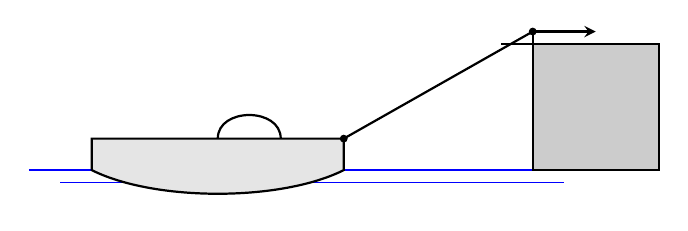
\begin{tikzpicture}[scale=0.8]
    % Agua
    \draw[blue, thick] (-1,0) -- (8,0);
    \draw[blue] (-0.5,-0.2) -- (7.5,-0.2);
    % Bote
    \draw[thick, fill=gray!20] (0,0) .. controls (1,-0.5) and (3,-0.5) .. (4,0) -- (4,0.5) -- (0,0.5) -- cycle;
    \draw[thick] (2,0.5) .. controls (2,1) and (3,1) .. (3,0.5); % Cabina
    \filldraw (4,0.5) circle (1.5pt); % Proa
    % Muelle
    \draw[thick, fill=gray!40] (7,0) rectangle (9,2);
    \draw[thick] (6.5,2) -- (9,2);
    \filldraw (7,2.2) circle (1.5pt); % Polea
    \draw[thick] (7,2) -- (7,2.2);
    % Cuerda
    \draw[thick] (4,0.5) -- (7,2.2);
    \draw[thick, -stealth] (7,2.2) -- (8,2.2);
\end{tikzpicture}
\end{center}
